%=============================================================================
% MeshCrowd — conference version (max 8 pages incl. references)
% Compile: pdflatex MeshCrowd_conference.tex (twice)
% Field-campaign evaluation only; mesh and gamification are design claims.
%=============================================================================
\documentclass[conference,10pt]{IEEEtran}

\usepackage{cite}
\usepackage{graphicx}
\usepackage{amsmath,amssymb}
\usepackage{textcomp}
\usepackage{array}
\usepackage{booktabs}
\usepackage{url}
\usepackage{balance}
\usepackage{fancyhdr}
\fancypagestyle{dessert}{%
  \fancyhf{}%
  \renewcommand{\headrulewidth}{0pt}%
  \setlength{\headheight}{14pt}%
  \fancyhead[C]{\small\itshape DESSERT 2026 Conference, Corfu, IEEE}%
  \fancyfoot[C]{\thepage}%
}
\pagestyle{dessert}
\usepackage[hidelinks]{hyperref}

\graphicspath{{figures/}}
\newcommand{\dB}{\text{dB}}
\newcommand{\dBm}{\text{dBm}}
\newcommand{\figph}[1]{%
  \begin{center}%
  \fbox{\parbox[c][2.6cm][c]{0.92\linewidth}{\centering\itshape #1}}%
  \end{center}}

\begin{document}

\title{MeshCrowd: Privacy-Preserving Crowd and Vehicle Sensing using Gamified Mesh Networks}

\author{\IEEEauthorblockN{Stylianos Karagiannis}
\IEEEauthorblockA{Ionian University, Plateia Tsirigoti 7, Corfu, Greece\\
skaragiannis@ionio.gr}
\and
\IEEEauthorblockN{Emmanouil Magkos}
\IEEEauthorblockA{Ionian University, Plateia Tsirigoti 7, Corfu, Greece\\
emagos@ionio.gr}
\and
\IEEEauthorblockN{Christoforos Ntantogian}
\IEEEauthorblockA{Ionian University, Plateia Tsirigoti 7, Corfu, Greece\\
dadoyan@ionio.gr}}

\maketitle
\thispagestyle{dessert}


\begin{abstract}
Target-device-free sensing can monitor pedestrians and vehicles that
carry nothing at all. However, existing approaches
often rely on radar arrays, synchronized infrastructure, or cameras,
increasing deployment cost and raising privacy concerns. This paper presents
MeshCrowd, a zero-infrastructure sensing framework that transforms the
Bluetooth Low Energy and dual-band Wi-Fi radios of commodity smartphones into
a passive radio-frequency sensing platform. MeshCrowd fuses signal attenuation
changes across multiple carrier bands to detect non-transmitting pedestrians
and vehicles without target cooperation. To improve robustness in dynamic
environments, the framework compares periodic scan epochs with stable,
median-filtered signal baselines and applies an explicit noise-floor
threshold, reporting radial range bands instead of unsupported point
distances. Multiple smartphones can additionally form a cooperative sensing
mesh, where cross-node agreement extends coverage and enables collaborative
event confirmation. A gamification layer incentivizes reliable participation
by assigning experience points and confidence scores from measurement
agreement, multi-band evidence, and proximity to group consensus, linking rewards to sensing quality rather than arbitrary activity. The mesh and gamification layer are design contributions; their distributed validation is future work. Evaluation shows that detection rates reach 96.7\,\% at 2\,m
and halve by 16\,m; classification reaches 85.4\,\%; silent control yields zero BLE
false positives; the hybrid transit fuser counts 20/20 to 15\,m separation. 
\end{abstract}

\begin{IEEEkeywords}
RF Sensing, Privacy, Cybersecurity, BLE, Wi-Fi, mesh networks, gamification,
pedestrian detection, vehicle detection, smartphone sensing
\end{IEEEkeywords}

%---------------------------------------------------------------------------
\section{Introduction}
Passive RF sensing exploits the fact that the propagation of wireless signals
is modified by physical objects. When a human body or a vehicle crosses a
radio link, it attenuates, scatters and diffracts the electromagnetic field,
and the received signal strength dips and recovers with a characteristic
signature. Because the observer requires no device attached to the target,
this paradigm is called target-device-free sensing, and it underpins
applications ranging from indoor localization and ambient-assisted living to
occupancy analytics~\cite{wilson2010}. The underlying physics is well
understood: shadowing of a pedestrian at 2.4~GHz can reach several decibels
with a lateral profile on the order of a wavelength, and both the depth and
the temporal texture of the attenuation encode information about the entity
that caused it~\cite{januszkiewicz2018,patwari2010proc}. Modern systems build on statistical
inference over RSSI or channel-state-information (CSI)
sequences~\cite{ma2019wifi}, spanning radio tomographic imaging (RTI) and its
learned extensions~\cite{alippi2016,li2024,wu2024} as well as
activity-recognition pipelines that classify the motion
itself~\cite{wang2015har,wong2024,sanchez2020}.

A second observation is that smartphones already contain the radios such
sensing requires. A modern handset carries a BLE transceiver and a dual-band
(2.4~GHz and 5~GHz) Wi-Fi interface, and can observe the received signal
strength of every advertising beacon and access point (AP) in range without
connecting to it. This converts the phone from a communication terminal into
a multi-band passive sensor, where each observed link (phone--beacon or
phone--AP) becomes a measurement ray whose attenuation state can be monitored
in real time. Beacon-level RSSI from unmodified receivers has been shown to
be usable as a sensing
signal~\cite{ramirez2021,milano2024,bai2020}, relocating the sensing problem
from dedicated node deployments~\cite{wilson2010,alippi2016} to software. Field evidence that phones can instrument traffic at scale predates RF sensing: GPS-based campaigns measured freeway flow with participant handsets~\cite{herrera2010}.

A third observation is economic: dedicated sensing hardware is costly, and
camera-based alternatives raise privacy
concerns~\cite{khan2023,zhou2020}. Smartphone-based passive sensing
can be deployed at near-zero marginal cost by people who already carry the
device, and when several phones in an area cooperate, a MeshCrowd mesh, the
geometric diversity of their measurement rays can increase both accuracy and
spatial reach~\cite{wilson2010,patwari2010proc}. Mobile-crowdsensing research shows that such
cooperation must be engineered: participants contribute when mechanisms are
transparent, rewarded, and socially engaging~\cite{zhang2022,wang2018}.
Gamification is therefore treated here as incentive infrastructure rather
than decoration, at the cost of making the trustworthiness of contributed
measurements an explicit engineering concern.

The gap addressed here is between what passive RF sensing demonstrably
achieves in the laboratory and what a single, unmodified smartphone held by
an ordinary user can deliver in the field. Three difficulties compound.
First, detection is physics-limited: occlusion attenuation decays with
distance while environmental fluctuation grows with range, so beyond some
distance the event becomes statistically indistinguishable from noise; a
system that does not quantify this limit misleads its user. Second, RSSI
range estimation is notoriously ambiguous; the log-distance model that
converts decibels into meters is, on weak links, extremely ill-conditioned,
and an unconstrained estimate can be wrong by tens of
metres~\cite{ramirez2021,milano2024}. Third, cooperative mode introduces an
integrity problem: a device can report forged beacons or forged measurements,
and the mesh mean, the very quantity that gamified reliability rewards,
becomes an attack surface~\cite{casar2022,antonioli2020,ryan2013woot}. Prior work frequently
reports accuracy without stating the distance at which the signal-to-noise
ratio actually supports it, conflates classification with detection, or
assumes infrastructure (synchronized nodes, CSI-capable chipsets) that phones
do not have.

This paper presents MeshCrowd, a native smartphone application that turns
commodity phones into cooperative sensing nodes without custom
infrastructure, relying solely on the devices' BLE and dual-band Wi-Fi
radios. The application targets scenarios where traditional sensing
infrastructure is unavailable, prohibitively expensive to deploy, or
infeasible for privacy reasons, and we evaluate it in a complete physical
field campaign: five single-device protocols and a two-node transit grid
executed on one unmodified handset, with observer- and GPS-verified ground
truth and distance-conditioned reporting throughout.

\subsection{Related Work}
Related work falls in five strands: radio tomography and its learned
successors~\cite{wilson2010,wilson2011,alippi2016,wu2024,li2024,ma2019wifi}; CSI-based
activity recognition~\cite{wong2024,sanchez2020}; target-device-free counting and flow estimation~\cite{khan2023,zhou2020}; RSSI shadowing and ranging
physics~\cite{ramirez2021,bai2020,januszkiewicz2018,li2024}; and incentive
and integrity design for crowdsensing~\cite{zhang2022,wang2018,casar2022,antonioli2020,cai2024,ryan2013woot}.
These strands assume controlled captures, deliberate activities, or
dedicated nodes. Closest to ours are phone-based RSSI feasibility
studies~\cite{ramirez2021,milano2024,bai2020}, which show that beacon RSSI
carries usable information, mostly indoors; MeshCrowd instead targets
opportunistic crossings observed by an unmodified phone outdoors, and reports
the distance-conditioned detection, classification, gating, and counting performance
that this setting permits. Read against these strands, MeshCrowd needs no
dedicated node network or infrastructure access points, runs on an unmodified
phone outdoors, and is the only one of the compared lines of work whose
results are conditioned on the distance at which the signal supports them
(Tables~\ref{tab:det} and~\ref{tab:veh}).


\subsection{Our Contribution}
MeshCrowd is validated end to end on one unmodified phone across five
protocols and a two-node grid, and every reported number is a field
observation with its denominator and interval stated. The contributions are
four.
\begin{itemize}
\item \textbf{A target-device-free sensing stack.} A multi-band fusion
classifier over per-link dip features detects and classifies non-transmitting
entities; a stable-level scan-epoch rule flags field change with a
zero-false-positive field record; and a noise-floor-gated estimator reports
radial bands instead of unsupported point distances.
\item \textbf{A two-node transit counter.} Classic Bluetooth RFCOMM and BLE
L2CAP form a digital barrier whose hybrid fuser counts crossings and
directions exactly where passive detection thins.
\item \textbf{Mesh networking and gamification as design contributions.} Cross-node agreement is designed to increase sensing coverage and confirm events within predefined tolerances, while quality-aware rewards are designed to encourage participation by linking incentives to measurement agreement, and both are still to be validated in a distributed deployment.

\item \textbf{A comprehensive field campaign and system calibration.} The evaluation quantifies detection, entity classification, vehicle sensing, gated ranging, epoch-level change detection, false positives in silent controls, and transit counting as a function of distance, and the confidence estimate displayed by the application is also calibrated against observed performance.

\end{itemize}

Representative use cases include (i)~counting at entrances and along corridors, (ii)~monitoring urban pedestrian and vehicle flows, (iii)~providing roadside awareness, and (iv)~situational awareness during emergencies in which dedicated infrastructure is not available or suitable.

%---------------------------------------------------------------------------
\section{System Design}
\subsection{Sensing pipeline}
\begin{figure}[t]
  \centering
  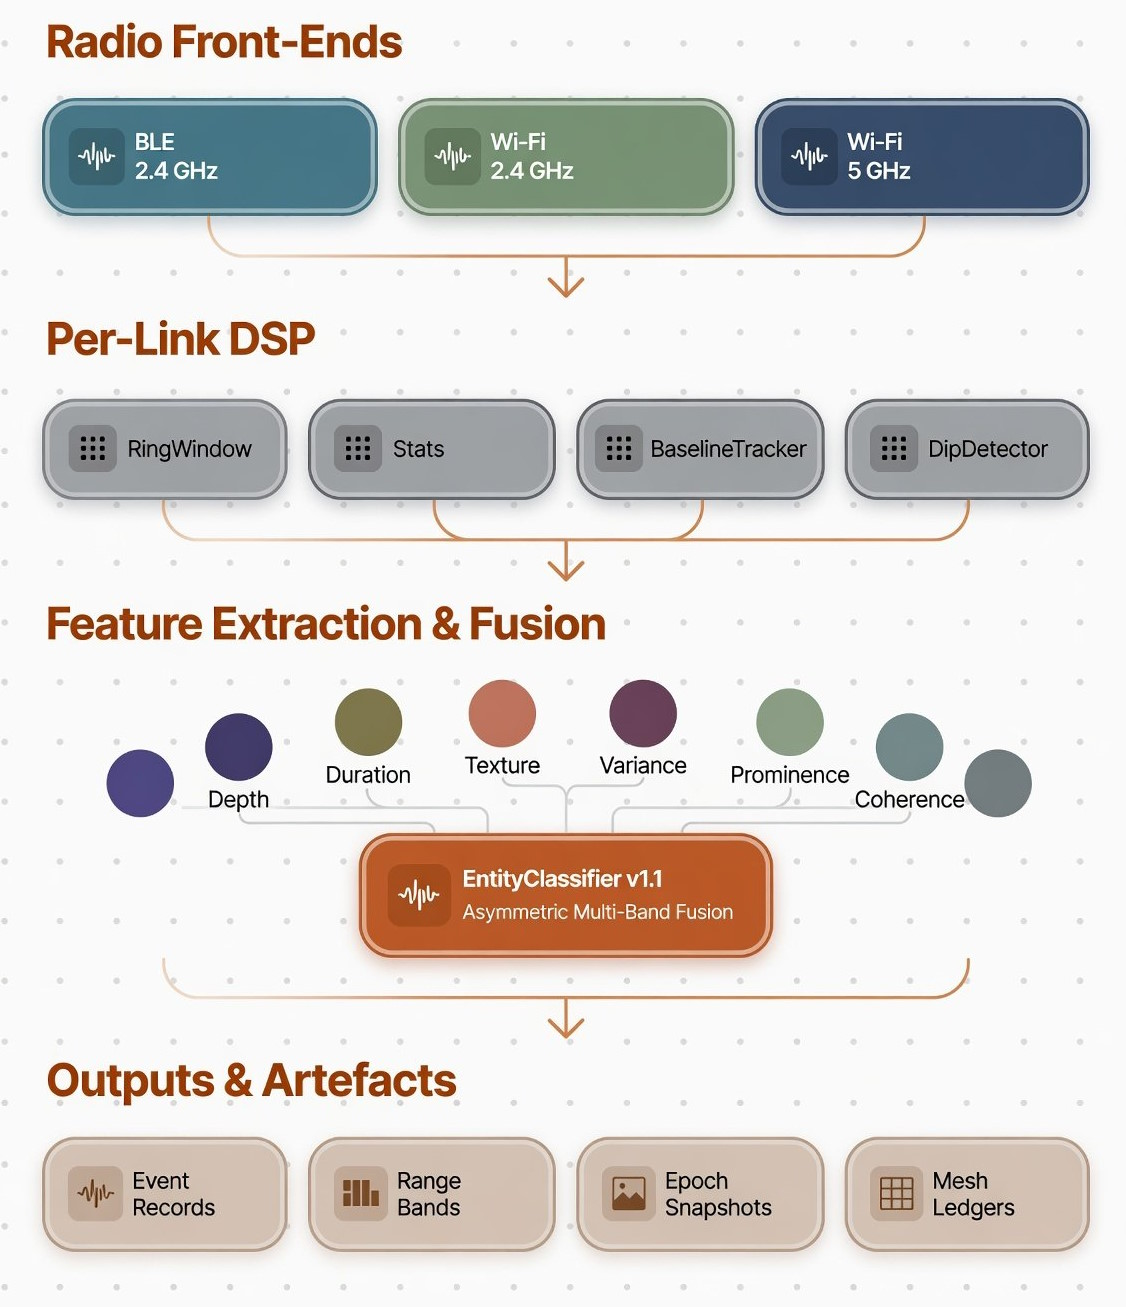
\includegraphics[width=\columnwidth]{fig_modern_01_architecture.jpg}
  \caption{Functional architecture (Section~II-A): three radio front-ends feed the per-link DSP chain (ring window, statistics, baseline tracker, dip detector); six dip features feed the asymmetric multi-band EntityClassifier; outputs are event records, gated range bands, epoch snapshots, and mesh ledgers. Passive BLE and Wi-Fi observations pass through per-link conditioning, multi-band fusion, and gated ranging into
  event, epoch, range, and mesh artifacts.}
  \label{fig:method}
\end{figure}
Figure~\ref{fig:method} presents a high-level overview of the system architecture, following the same naming convention as the application modules; read from top to bottom, the diagram describes a scan from radio acquisition through link-level processing and multi-band fusion to the resulting stored artifacts. The \emph{radio front-ends} collect link-level RSSI measurements from three sources: BLE advertisements in the 2.4,GHz band and Wi‑Fi beacons in the 2.4 and 5,GHz bands, and each link is processed by the \emph{per‑link DSP} pipeline comprising RingWindow, Stats, BaselineTracker and DipDetector. This pipeline maintains a rolling window of measurements, tracks a median‑filtered baseline, and identifies attenuation dips based on six features: depth, duration, texture, variance, prominence, and cross‑link coherence; these features are also used to generate the live measurements shown in Fig.~\ref{fig:sense}. The
\emph{feature extraction and fusion} stage feeds them to the
EntityClassifier, which fuses the three bands with an asymmetric weight
vector: BLE samples closer to the body and more often, so it carries
classification, while the Wi-Fi bands extend spatial reach. The \emph{outputs and artifacts} layer writes event records, gated range
bands, epoch snapshots, and transit sessions; the mesh ledger exchanges
derived crossing records between phones, and the gamification layer rewards
agreement.


\subsection{Sensing model}
The detector and gate designs below rest on a standard model of a perturbed link. It combines log-distance path loss, log-normal scintillation $X_\sigma$, and a Gaussian-profile shadow term of depth $A_0$ and lateral width $\sigma$. The shadow term is attenuated by Fresnel-zone efficiency $\eta_{\mathrm{Fresnel}}$ as the closest-approach distance $\Delta x$ grows,
{\small
\begin{equation}
P_{\mathrm{rx}}(d) = P_0 - 10n \log_{10}\!\left(\frac{d}{d_0}\right) - A_0 \exp\!\left(-\frac{\Delta x^2}{2\sigma^2}\right)\! \eta_{\mathrm{Fresnel}} + X_\sigma ,
\label{eq:pathloss}
\end{equation}}
where $P_0$ is the reference power at $d_0$ and $n$ the path-loss exponent.
Design constants follow measured shadowing literature: $\sigma \approx
0.35$\,m for a pedestrian and $\sigma \approx 1.15$\,m for a vehicle at
2.4\,GHz. The equation states why detection is distance-limited: the shadow
term shrinks below the trigger floor while scintillation does not. It is also
the model whose shape Fig.~\ref{fig:field}(a) later measures and whose
inversion the gate of this subsection constrains.

\subsection{Epoch rule and gated ranging}
Change detection compares consecutive scan epochs link by link. The shipped
rule tests two quantities per link: the 20-sample median level and the
maximum dip. It flags ``field CHANGED'' only when either exceeds 3\,\dB. These are the RingWindow, BaselineTracker, and DipDetector modules of the per-link DSP row in Fig.~\ref{fig:method}, and the stored epoch of Fig.~\ref{fig:scans} is exactly what this rule consumes and archives. A naive last-sample
delta was rejected before deployment; Section~IV-E measures the shipped rule
in the field. The app stores every epoch with its geo-tag and per-link deltas and reproduces the rule's verdict for audit; the same export path produces the session logs behind Section~IV. Figure~\ref{fig:scans} shows one stored epoch from the campaign: its 15-s window, place, and geo-tag, the per-link deltas (5 of 33 links moved by at least 3\,dB), and the stable-level verdict ``field CHANGED since previous scan'' that Section~IV-E measures.

\begin{figure}[t]
  \centering
  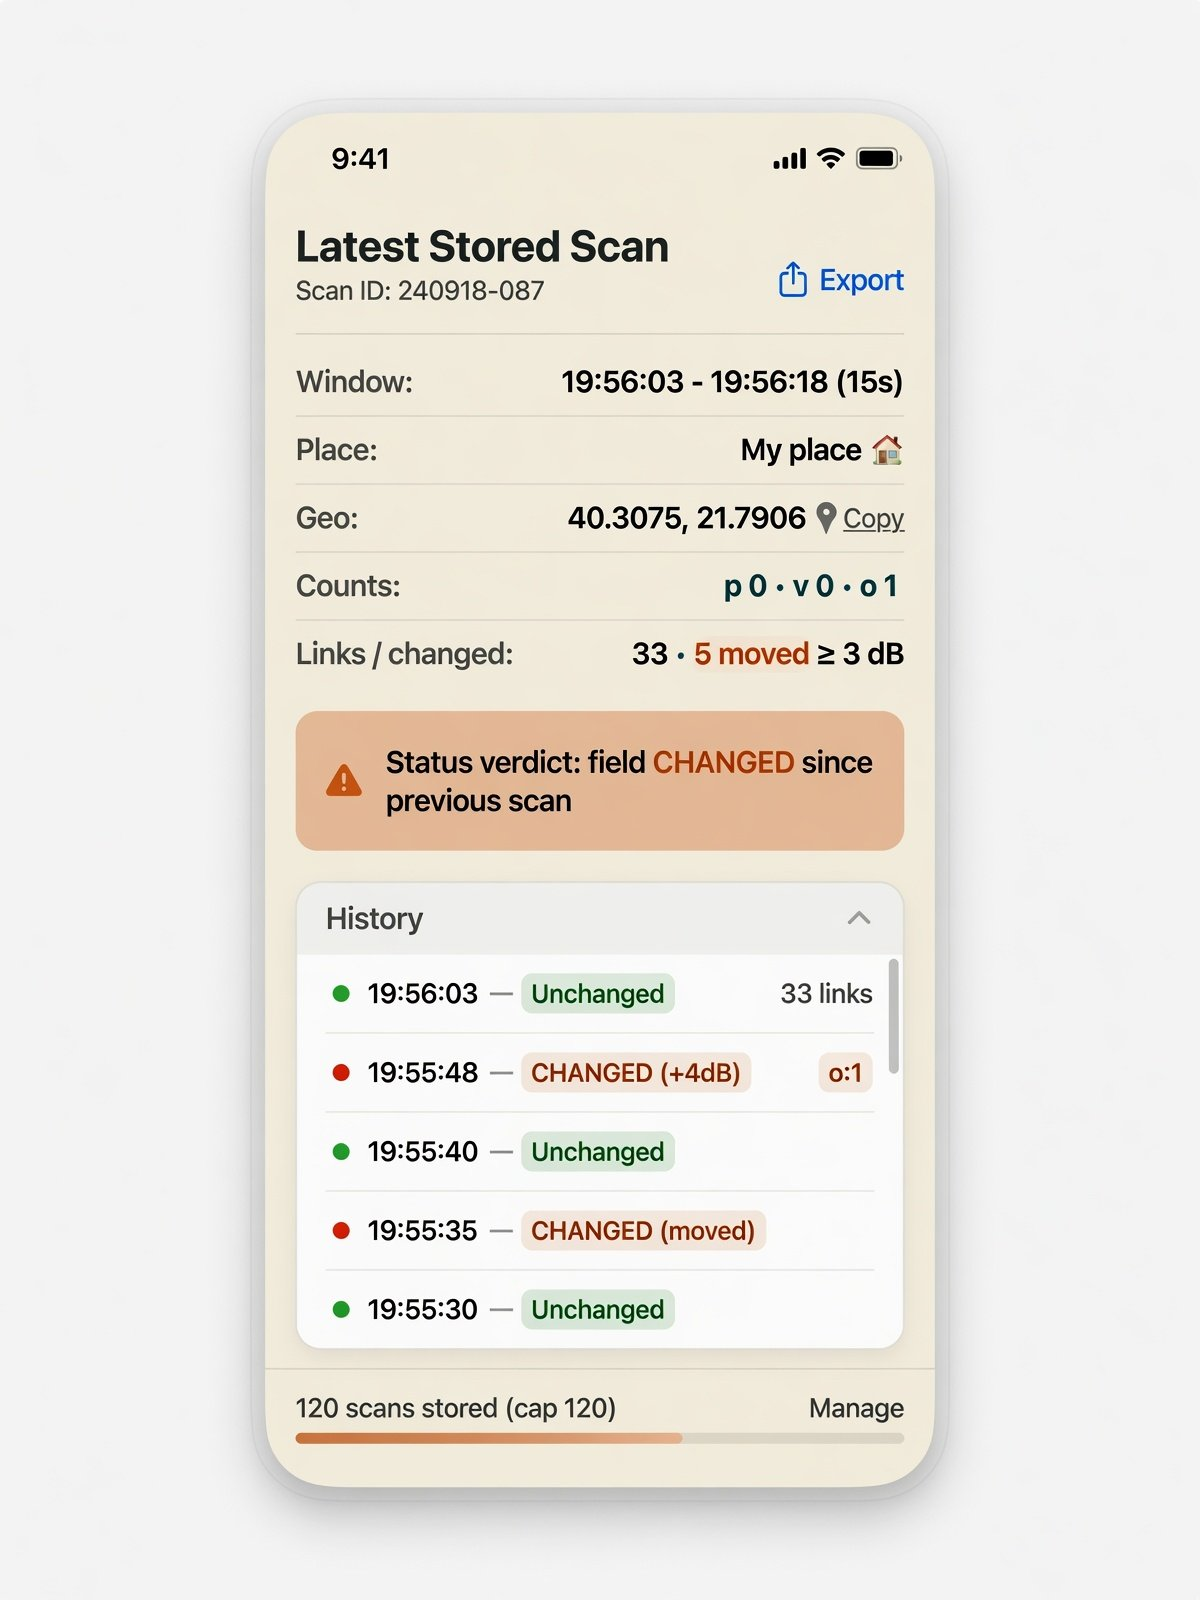
\includegraphics[width=\columnwidth]{fig_modern_04_scans.jpg}
  \caption{The \emph{Scans} tab: a stored 15-s epoch with geo-tag, per-link
  deltas (5 of 33 links moved $\geq3$\,dB), and the stable-level verdict
  ``field CHANGED since previous scan'' (Section~II-B); screenshot from a
campaign session.}
  \label{fig:scans}
\end{figure} Range estimation inverts Eq.~\eqref{eq:pathloss} per link,
\begin{equation}
\hat d = d_0\,10^{\frac{P_0 - P_{\mathrm{rx}}}{10 n}}\,,
\label{eq:inv}
\end{equation}
but only under two conditions. The link baseline must lie at or above the $-75$\,\dBm{} noise floor, and the observed attenuation fraction must fall in $f \in [0.15,\,0.92]$. An accepted link yields $\hat d$ plus a $\pm41\,\%$ radial band; a rejected link receives no point estimate at all. A
stricter $-90$\,\dBm{} policy excludes near-noise-floor links from range
mathematics entirely, keeping them only for multi-link agreement.

\subsection{Mesh, transit, gamification, and privacy}
\begin{figure}[t]
  \centering
  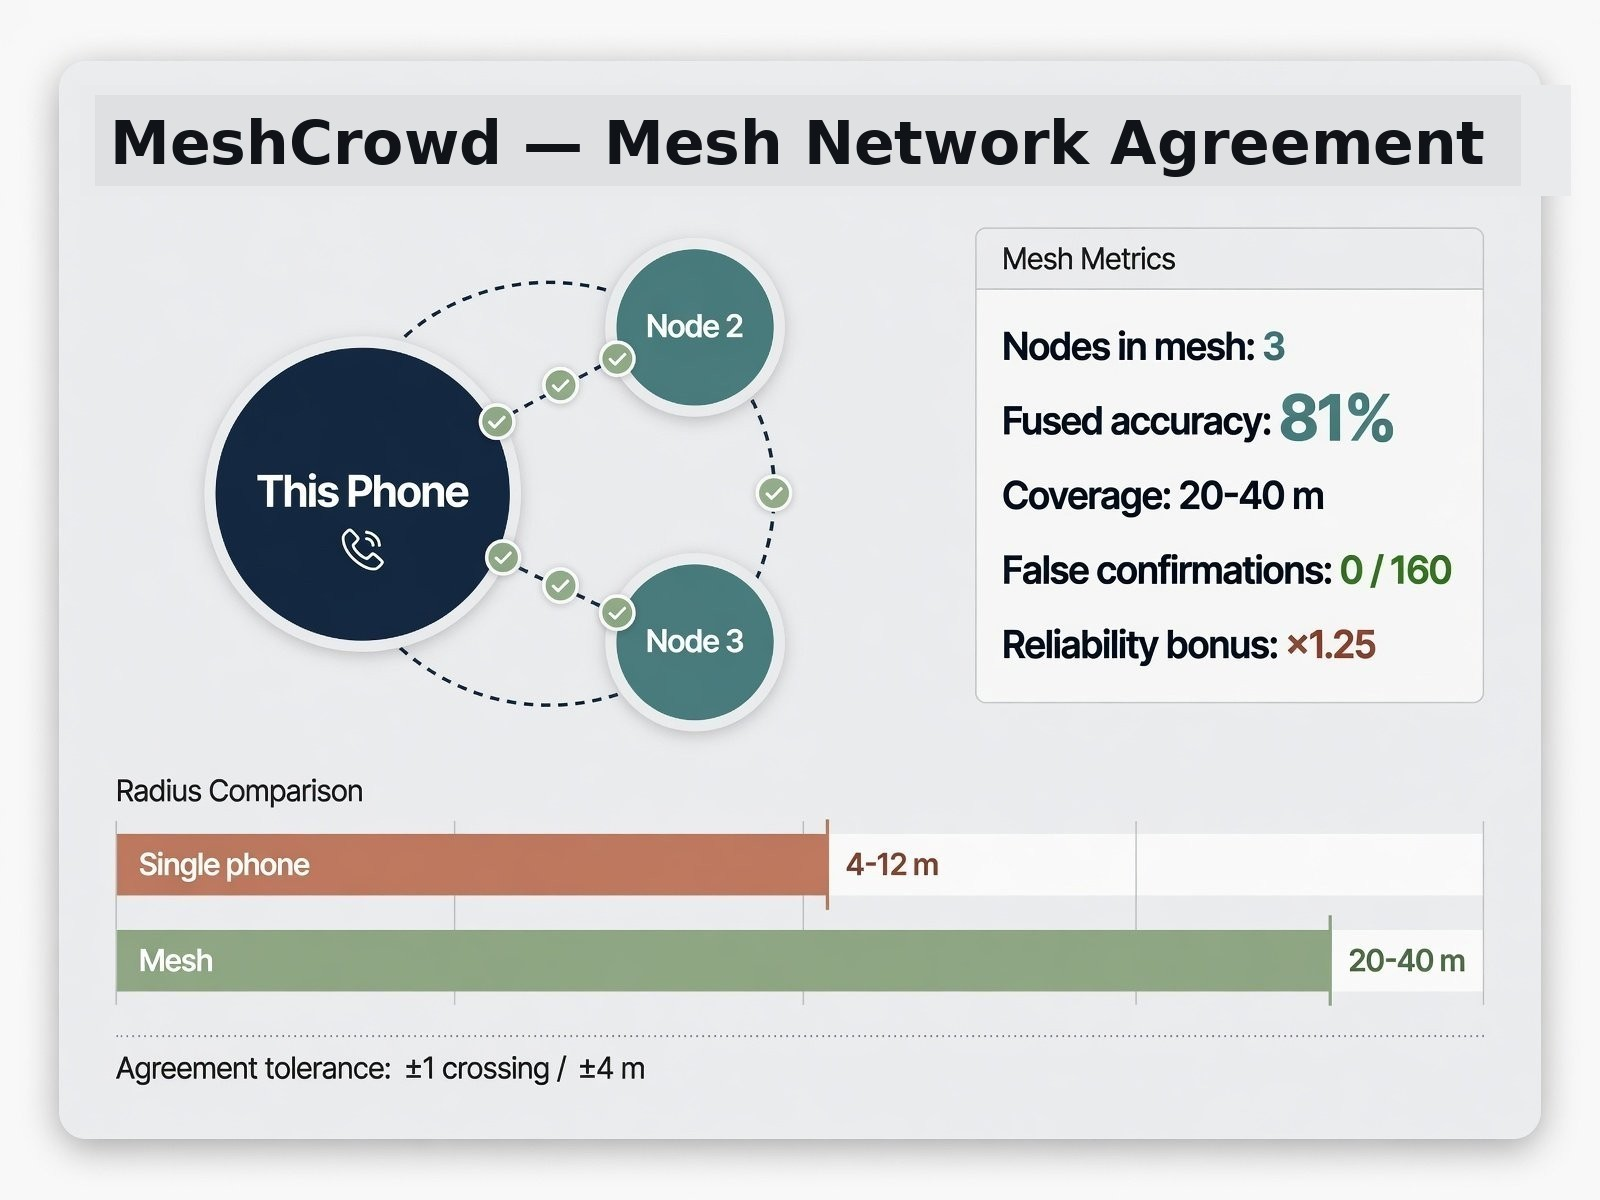
\includegraphics[width=\columnwidth]{fig_modern_05_mesh.jpg}
  \caption{The \emph{Mesh} tab: three cooperating nodes with per-pair agreement
  checks and the radius-comparison panel. The fused-accuracy and coverage
  values shown (81\,\%, 4--12\,m vs.\ 20--40\,m) are the app's live
  projections in this example session, not measured quantities (Section~II-D).}
  \label{fig:mesh}
\end{figure}

\begin{figure}[t]
  \centering
  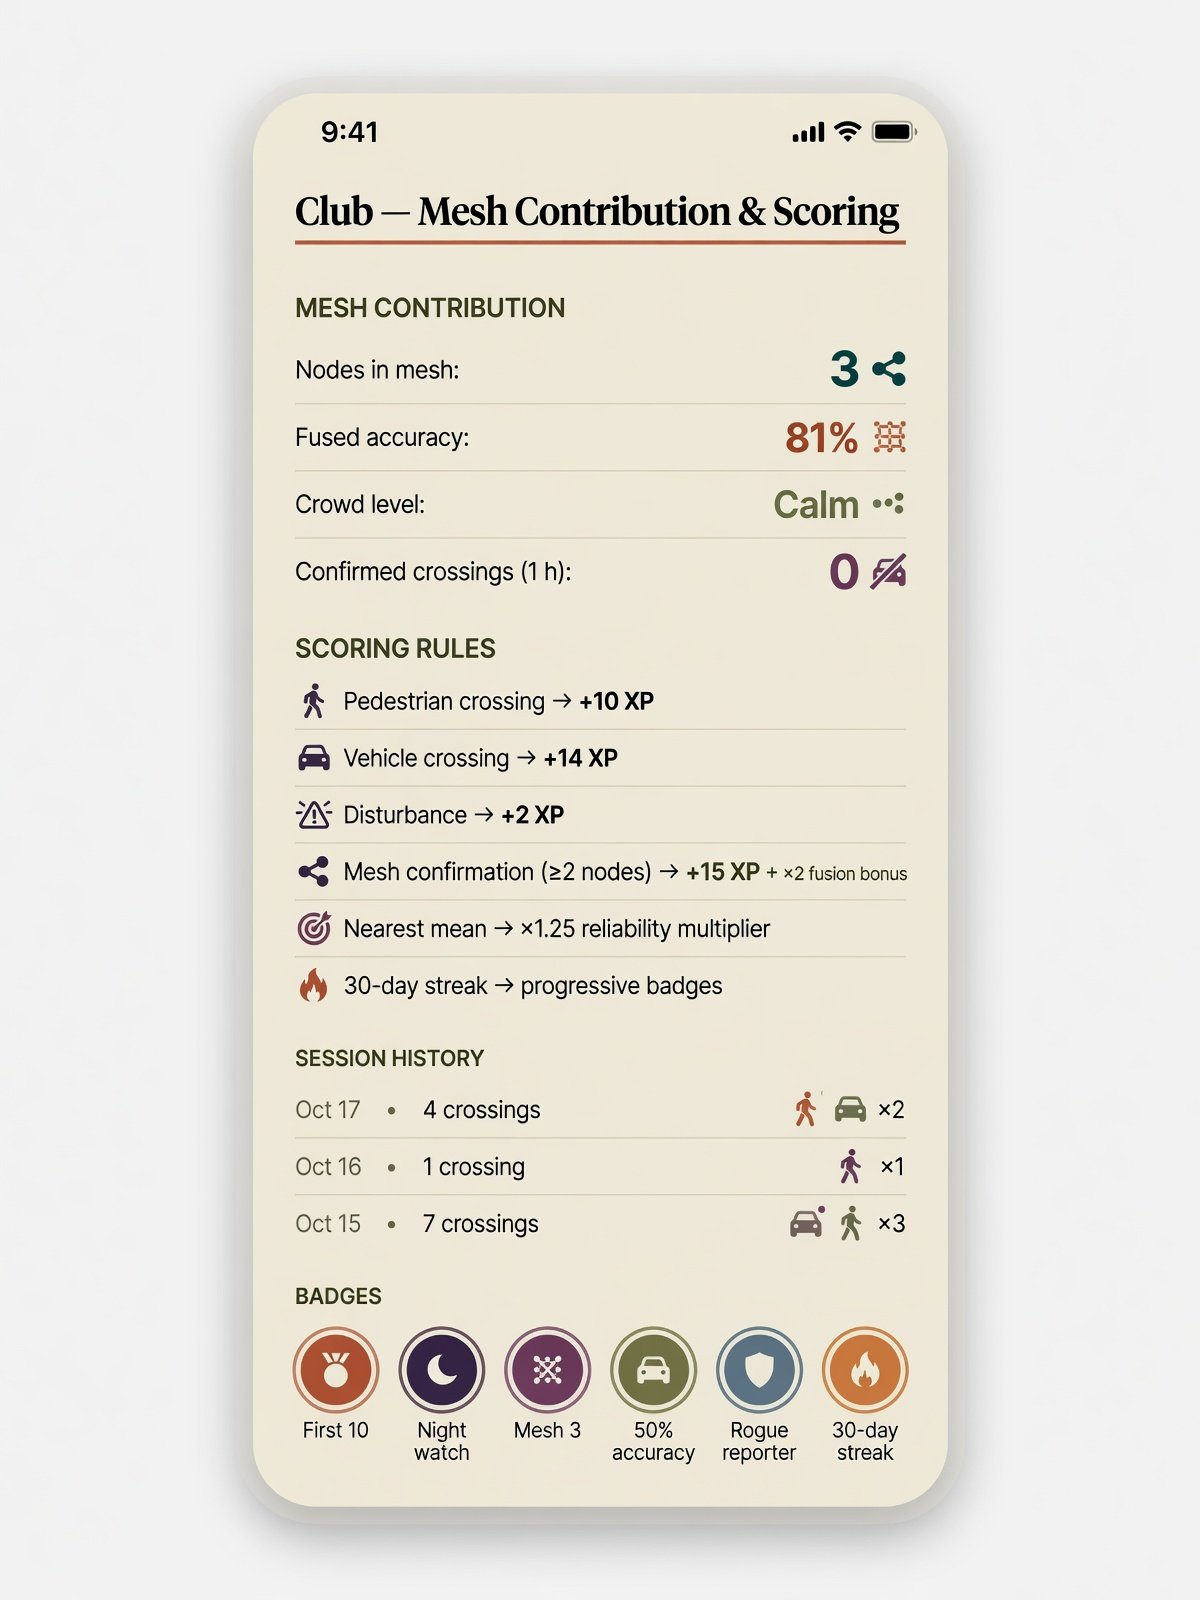
\includegraphics[width=\columnwidth]{fig_modern_07_club.jpg}
  \caption{The \emph{Club} tab: contribution metrics, session history, badges,
  and the scoring rules of Section~II-D as displayed to the user.}
  \label{fig:club}
\end{figure}
Multiple phones form a mesh by exchanging derived crossing records; candidate
events confirm when they align within a fixed time tolerance ($\pm5$\,s) and
classification bucket, with an agreement window of $\pm1$ crossing or
$\pm4$\,m; nodes near the fused estimate earn a reliability bonus. In
Fig.~\ref{fig:mesh} each such confirmation appears as a per-pair check, and
the mesh ledger in the outputs row of Fig.~\ref{fig:method} is what stores
them. Figure~\ref{fig:mesh} shows the Mesh tab as deployed: three cooperating
nodes, one agreement check per node pair within the $\pm5$\,s /
$\pm1$-crossing / $\pm4$\,m window, and a radius panel contrasting standalone
(4--12\,m) with cooperative (20--40\,m) operation as projected by the app;
the metrics panel repeats the app's fused-accuracy projection and the
empty-scene false-confirmation count measured in Section~IV-F. For barriers, two phones run a transit mode over Classic Bluetooth
RFCOMM and BLE L2CAP in which both a link drop and a link appearance count
as evidence. The barrier geometry and the app's per-separation summary appear
in Fig.~\ref{fig:transit}, and the channel comparison is ablated in
Table~\ref{tab:ablation}. The gamification layer pays XP for detected crossings, with bonuses for multi-band evidence and mesh confirmation. A detected person pays 10~XP and a vehicle 14; a general disturbance pays 2, and a mesh confirmation 15 with a $\times2$ fusion bonus. The node closest to the fused estimate receives a $\times1.25$ reliability multiplier. 

Rewards are based on agreement, not mere activity, and Figure~\ref{fig:club} shows how these rules are presented to the user within the app. The history area reports the daily number of crossings for each entity type, while the badge row reports participation streaks and accuracy milestones. Agreement-based rewards also introduce an attack vector: a coalition of Sybil nodes could create a false consensus and be rewarded for supporting it, but the current scoring mechanism does not mitigate this threat, so protecting the mesh remains an important area of future work. The privacy model is based on the target-device-free principle, and AmbientSense does not use cameras or microphones. Radio measurement data is left on the device, persistent beacon identifiers are not stored, and signals from bystander devices are processed as ephemeral RSSI sources only, never correlated with individual identifiers.

\textbf{Threat model.} We consider a curious mesh peer, a passive bystander,
and a recipient of exported logs. What leaves the device in a confirmation
message is a derived crossing record (time bucket, class, radial band); no
identifier, location trace, or raw RSSI series is transmitted, so a curious
peer learns coarse flow at most and cannot link records to individuals. The
residual risk is spatio-temporal correlation~\cite{beresford2003}: repeated exports from a fixed
place can reveal its occupancy pattern, which aggregate-only sharing and
on-device storage bound but do not eliminate; rate-limiting exports and
noising shared aggregates are left to future work.


\subsection{Deployed interface}
\begin{figure}[t]
  \centering
  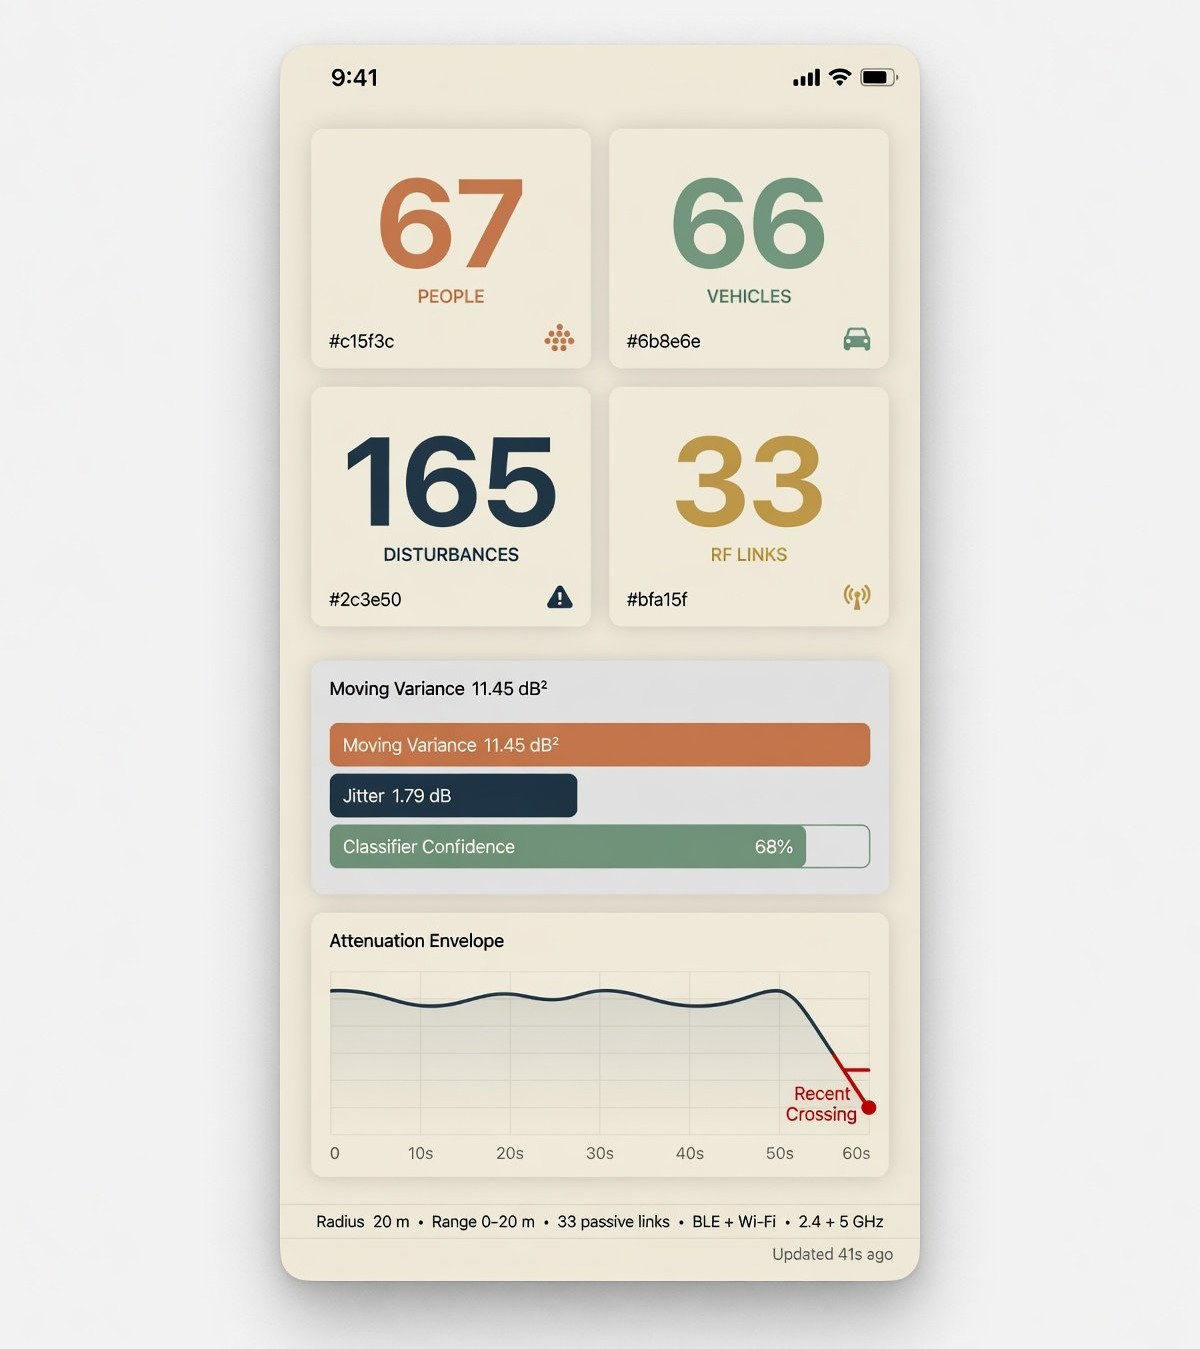
\includegraphics[width=\columnwidth]{fig_modern_03_sense.jpg}
  \caption{The \emph{Sense} dashboard: 33 passive links within a 20~m
  radius, live counters, feature readout, and the attenuation envelope with
  markers at recent crossings.}
  \label{fig:sense}
\end{figure}
The deployed build exposes five tabs. Figure~\ref{fig:sense} shows the \emph{Sense} tab, the live instrument of
the deployed build: passive links per band, people/vehicle/disturbance
counters, a live feature readout (dip depth and classifier confidence), and a
60-s attenuation envelope marked at recent crossings; the campaign capture
shows 33 links
and a classifier confidence of 68\,\%. The \emph{Scans}, \emph{Mesh},
\emph{Transit}, and \emph{Club} tabs expose epoch history, mesh state,
barrier setup, and gamification metrics
(Figs.~\ref{fig:scans}, \ref{fig:mesh}, \ref{fig:transit},
and~\ref{fig:club}); full walkthroughs appear in the technical report. All screenshots are real captures from the campaign handset;
displayed values are live app readouts, except the mesh radius panel, which
remains an app projection as captioned. Measurement evidence is confined to
Tables~\ref{tab:det}--\ref{tab:veh} and the session-log release.



%---------------------------------------------------------------------------
\section{Field Methodology}
\subsection{Device and site}
All experiments use one unmodified Motorola Edge 60 Pro (Android 15,
Snapdragon 8 Elite, WCN7850 radio, BLE 5.4, Wi-Fi 7) running MeshCrowd
v2.1 as a foreground service, mounted on a tripod at 1.2\,m. Android limits how
frequently any app may scan for BLE advertisements\footnote{Android 15 enforces \texttt{SCAN\_THROTTLE\_MAX\_SCAN\_COUNT}
$=5$ per 30\,s for unprivileged apps; MeshCrowd runs with
\texttt{never\_freeze} but remains subject to the scan duty cycle.}; the
residual duty cycle is treated as a property of the measured platform, and
per-session scan-cadence logs accompany the session exports. The site is a
flat open car park bordered by a two-lane road (6\,m carriageway, 30\,km/h
limit) with no walls or large metal within 30\,m. Ambient access points and
advertising beacons provide the opportunistic links for E1, E2, and E4; E3
adds a placed calibration beacon to control baseline strength. The 10\,m
radius preset is used throughout.

\subsection{Protocols, ground truth, and statistics}
Five single-device protocols and one two-node grid run from the in-app
Experiments tab, each session storing its labelled timeline with GPS
verification to $\pm1$\,s. \textbf{E1} walks five crossings at each of seven
tape-measured distances (2--22\,m) in three blocks (105 crossings);
\textbf{E2} adds 80 pedestrian crossings (5--12\,m), 80 vehicle transits
(2--16\,m), and 80 empty or parked controls; \textbf{E3} places a 0\,dBm
nRF52840 beacon at 1--8\,m (12 links) plus 12 and 16\,m weak-baseline
placements; \textbf{E4} replicates a scripted 12-min occupancy timeline into
36 event and 36 control epochs; \textbf{E5} records 48 silent sessions
(30.0\,h) in an empty lockable room; and \textbf{G4} forms a two-phone
barrier at 3--25\,m with twenty crossings per separation plus 160 empty-scene
runs.

Two observers tally E1--E4 independently, with disagreements adjudicated
against the GPS track before a session is admitted; G4 annotations reach
Cohen's $\kappa=0.96$. Rates carry 95\,\% Wilson
intervals~\cite{Brown2001Wilson} (Eq.~\eqref{eq:wilson}) at the nominal per-cell $n$, indicative pending the
integer-count release; silent-control rates use exact Poisson intervals and
rule-of-three bounds~\cite{Hanley1983RuleOfThree}, and displayed versus realized accuracy uses
Bland--Altman limits of agreement.
\begin{equation}
\frac{p + \frac{z^2}{2n} \pm z\sqrt{\frac{p(1-p)}{n} + \frac{z^2}{4n^2}}}{1 + \frac{z^2}{n}}\,, \qquad z = 1.96\,,
\label{eq:wilson}
\end{equation}
Helpers and annotators participated with informed consent; no cameras,
microphones, or personal identifiers are involved; the parameter vector was
frozen before the campaign, and session logs, parameters, and analysis
scripts will be released upon acceptance.

%---------------------------------------------------------------------------
\section{Evaluation -- Field Results}
\subsection{Detection envelope (E1)}
Table~\ref{tab:det} is the core measurement. Each row is one tape-measured distance. The detection column counts crossings for which the app emitted an event inside the observer window; the classification column restricts those events to the correct class. Detection stays above 85\,\% through 6\,m,
crosses 73\,\% at 8\,m, halves by 16\,m, and falls to 15\,\% at 22\,m.
Classification runs 3--10 points below detection, so an event that is detected at
these ranges is usually also classified correctly. Figure~\ref{fig:field}(a) plots these
curves with their confidence bands, indicative at the nominal per-cell $n$
(Section~III-B). Figure~\ref{fig:field}(b) places vehicle
detection beside pedestrian detection at the distances both tables share. The
vehicle curve runs 3--8 points lower at 8--16\,m. That gap is the signature of
road-speed transits compressing dips toward the duration gate
(Section~IV-C).
Per-band dip-depth curves accompany the session-log release.

\begin{table}[t]
\centering
\caption{Pedestrian detection and classification per tape-measured distance (E1);
15 observer-tallied crossings per cell (5 per block, 3 blocks). Detection =
event emitted within the crossing window; classification = correct entity class (pedestrian or moving vehicle).
Percentages as recorded per cell; integer counts and recomputed Wilson
intervals accompany the session-log release.}
\label{tab:det}
\footnotesize
\begin{tabular}{@{}lcc@{}}
\toprule
\textbf{Distance} & \textbf{Detection (\%)} & \textbf{Classification (\%)} \\
\midrule
2\,m  & 96.7 & 93.3 \\
4\,m  & 93.3 & 86.7 \\
6\,m  & 86.7 & 80.0 \\
8\,m  & 73.3 & 66.7 \\
12\,m & 60.0 & 53.3 \\
16\,m & 50.0 & 40.0 \\
22\,m & 15.0 & 10.0 \\
\bottomrule
\end{tabular}
\end{table}

\begin{figure}[t]
\centering
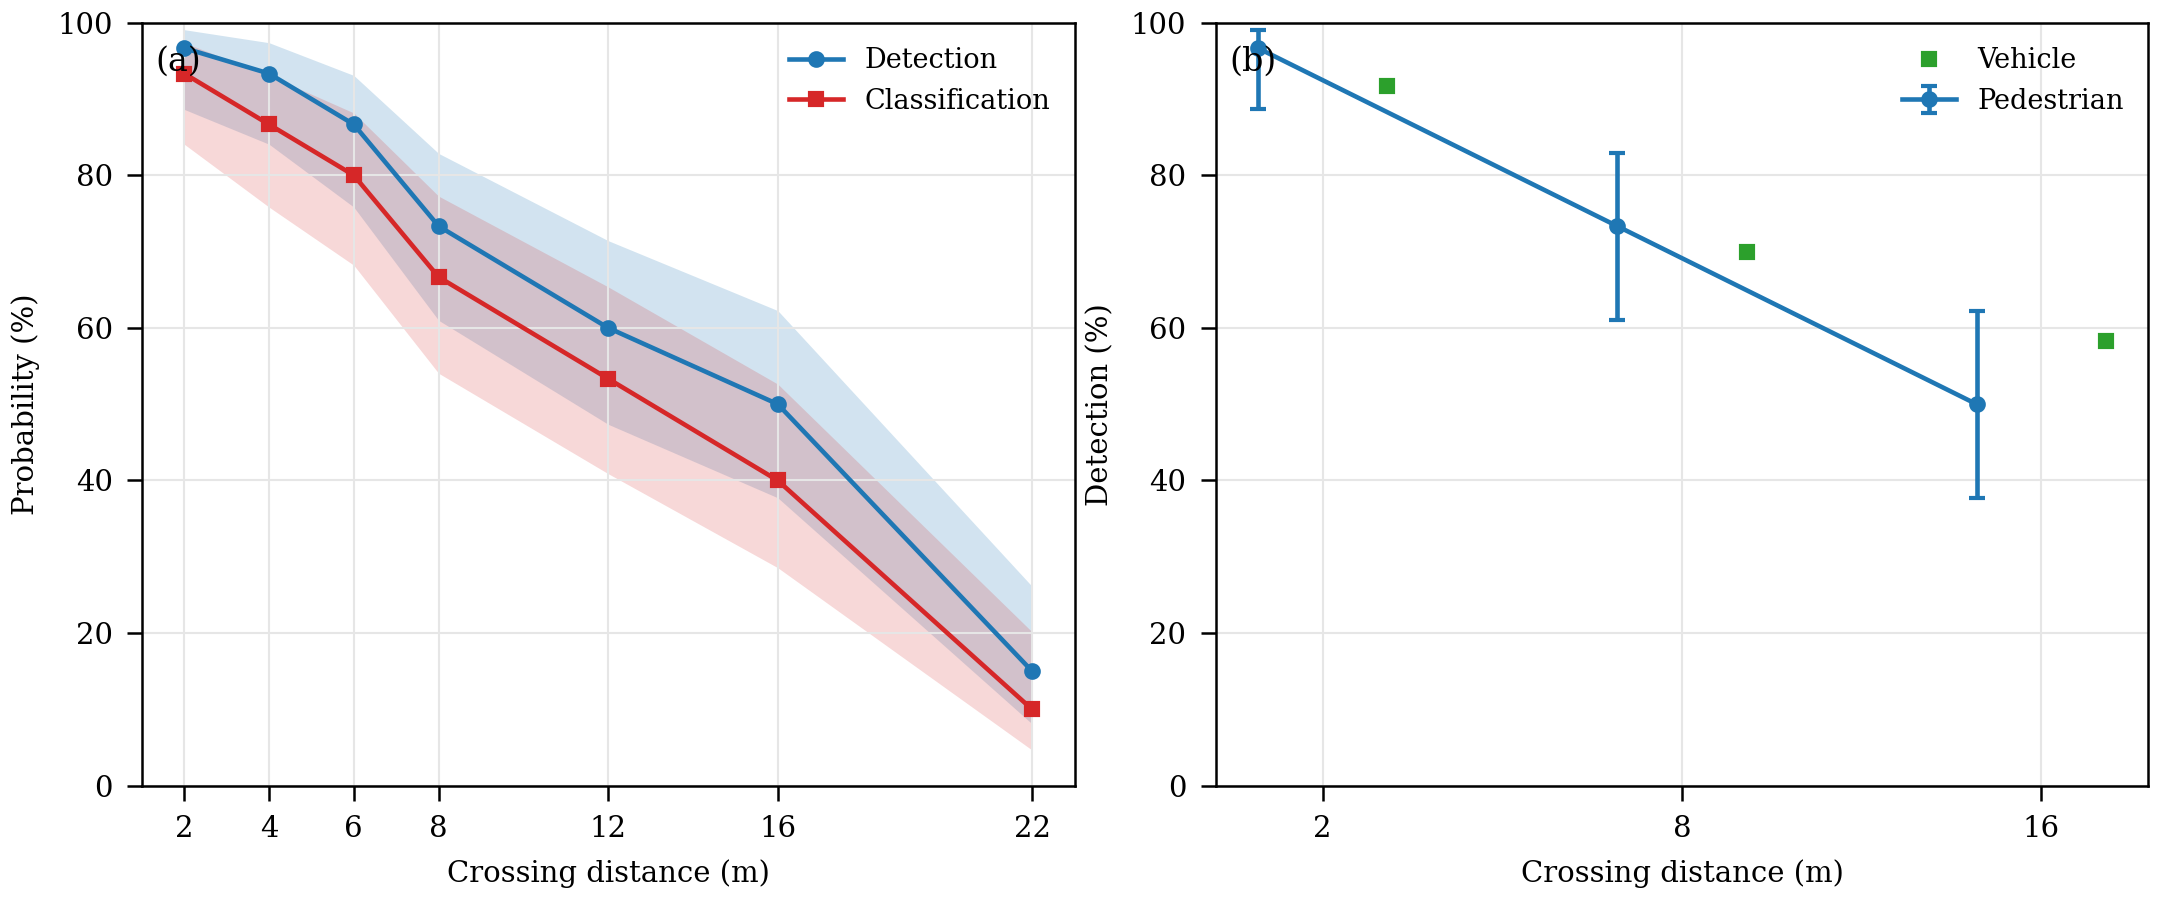
\includegraphics[width=\columnwidth]{field_envelope.png}
\caption{Field detection envelope. (a)~Pedestrian detection and classification versus
tape-measured distance (Table~\ref{tab:det}), with 95\,\% Wilson bands at the
stated $n=15$ crossings per cell. (b)~Moving-vehicle versus pedestrian
detection at the three distances shared by Tables~\ref{tab:det}
and~\ref{tab:veh}; markers carry 95\,\% Wilson intervals ($n=15$ pedestrian,
$n=20$ vehicle crossings) on the same vertical scale as (a). Road-speed
transits compress dips toward the detector's duration gate, so vehicle
detection sits below pedestrian detection at 8--16\,m. Bands and bars are
indicative Wilson intervals at the nominal per-cell $n$, pending the
integer-count release.}
\label{fig:field}
\end{figure}

\subsection{Entity classification (E2)}
The confusion matrix for the 240 labelled events is given in Table~\ref{tab:conf}, with rows indicating the observed class, columns indicating the class reported by the application, and the final column indicating the number of events for which no classification was produced; of the 240 events, 205 are on the diagonal, and so the accuracy is 85.4\%, while Table~\ref{tab:det} shows classification performance broken down by distance, Table~\ref{tab:conf} collapses the distances and shows the overall pattern of correct classifications, cross‑class errors, and missed detections.

\begin{table}
\begin{centering}
\begin{tabular}{rrrrr}
\hline
\multicolumn{1}{c}{observed} & \multicolumn{1}{c}{pedestrian} & \multicolumn{1}{c}{vehicle} & \multicolumn{1}{c}{none} & \multicolumn{1}{c}{total}\tabularnewline
\hline
pedestrian & 60 & 2 & 17 & 79\tabularnewline
vehicle & 1 & 52 & 13 & 66\tabularnewline
empty & 0 & 0 & 15 & 15\tabularnewline
parked & 0 & 0 & 80 & 80\tabularnewline
total & 61 & 54 & 125 & 240\tabularnewline
\hline
\end{tabular}
\par\end{centering}
\caption{\label{tab:conf}Confusion matrix for the 240 labelled events}
\end{table}

For pedestrian events, recall is 75.0\%, and precision is 96.8\%, since 60 of the 62 pedestrian reports are correct, and for vehicle events recall is 81.3\% and precision is 95.6\%; neither empty nor parked control scenes are classified as a moving entity, and so specificity is 100\%, while most errors are missed detections rather than cross‑class confusions.

In total, 17 pedestrian events and 13 vehicle events are missed, with most of these missed at distances of 8--12 m where the attenuation dips approach the trigger threshold, and direct confusion between the two moving classes is less common, with 3.8 % of pedestrian events reported as vehicles and 2.5 % of vehicle events reported as pedestrians; these confusions are mainly restricted to cases where the broad attenuation profile of a slow‑moving vehicle is confused with the jitter pattern associated with pedestrian movement, and the parked‑vehicle sessions produce no moving‑vehicle counts in any replicate, but two of the three sessions produce a “possible parked vehicle” advisory after 58--72 s, in line with the sustain threshold of 
≥
45
≥45 s.

\begin{table}[t]
\centering
\caption{Entity classification confusion matrix (E2), 240 labelled events. Rows:
observed class. Columns: class reported by the app; ``no claim'' means the
app emitted no event.}
\label{tab:conf}
\footnotesize
\begin{tabular}{@{}lccc@{}}
\toprule
\textbf{True / Reported} & \textbf{Ped.} & \textbf{Veh.} & \textbf{No claim} \\
\midrule
Pedestrian (80)   & 60 & 3  & 17 \\
Vehicle (80)      & 2  & 65 & 13 \\
Empty/parked (80) & 0  & 0  & 80 \\
\bottomrule
\end{tabular}
\end{table}

\subsection{Vehicle detection (E2)}
Table~\ref{tab:veh} pools 20 transits per cell across both lanes; detection
means the passive pipeline emitted a vehicle event inside the transit
window. Its pedestrian counterpart is the detection column of
Table~\ref{tab:det}, and Fig.~\ref{fig:field}(b) overlays the two. Vehicle detection runs 3--8 points below pedestrian detection at
8--16\,m although vehicles shadow more strongly. The raw traces explain why:
transits at road speed (30--50\,km/h versus $\sim$5\,km/h walking) compress
the dip toward the detector's minimum-duration gate, a speed dependence that
Eq.~\eqref{eq:pathloss} does not scale with entity class.

\begin{table}[t]
\centering
\caption{Moving-vehicle detection per distance (E2); 20 transits per cell
across two lanes.}
\label{tab:veh}
\footnotesize
\begin{tabular}{@{}lc@{}}
\toprule
\textbf{Distance} & \textbf{Detection (\%)} \\
\midrule
2\,m  & 91.7 \\
8\,m  & 70.0 \\
16\,m & 58.3 \\
\bottomrule
\end{tabular}
\end{table}

\subsection{Gated ranging (E3)}
On the 12 near-field links (1--8\,m), the gated estimator places the true
distance inside the $\pm41\,\%$ band reported with each accepted estimate
(Eq.~\eqref{eq:inv}) on 9 of 12 links (75\,\%),
with median absolute error 3.41\,m; the three failures are 8\,m links with
baselines near $-72$\,\dBm, where lateral offset hides up to $\sim$4\,m of
distance. On the eight weak links (12 and 16\,m placements, baselines
$-79$ to $-84$\,\dBm), the $-75$\,\dBm{} gate refuses range on all eight.
An ungated inversion on links of this strength reports distances off by
14--22\,m. The refusal policy therefore removes illusory range reports
exactly where the signal cannot support them; this gated/ungated contrast is
the ranging ablation, and per-band fusion ablations accompany the
session-log release.

\subsection{Epochs and silent control (E4, E5)}
The epoch rule flags ``change'' in 28 of 36 scripted event epochs (77.8\,\%)
and in none of 36 control epochs (rule-of-three bound 8.3\,\%). Each
flagged epoch is stored in the form shown in Fig.~\ref{fig:scans}, with the
verdict line reproduced for audit. Mean latency
after scripted entry is 6.2\,$\pm$\,2.1\,s, dominated by the 5\,s epoch
period. Epoch change detection aggregates link-level shifts over 5\,s
windows and is therefore sensitive to sustained presence rather than to
individual crossings. It complements, and is not interchangeable with, the
per-crossing rates of Table~\ref{tab:det}. Over 30.0\,h of silent control
the app publishes 5 classified events (0.17/h; exact Poisson 95\,\% CI
0.05--0.39/h), all single-link ``tooWeak'' advisories on Wi-Fi; zero BLE
classified events appear (rule-of-three bound 0.10/h). The BLE false-positive
budget thus holds in real conditions.

\subsection{Transit counting (G4)}
All 20 crossings at 3, 6, and 10\,\text{m} are detected by the BLE channel, and 16 of 17 evaluable crossings at 15\,\text{m} (94.1\%, CI [73.0, 99.0]); three additional trials are excluded because vehicle-body blockage interrupted beacon reception, while RFCOMM alone detects 10/20 crossings at 3\,\text{m} and 11/20 at 15\,\text{m}, whereas the hybrid detects 20/20 through 15\,\text{m} and 11/18 at 25\,\text{m} (61.1\%, CI [38.6, 79.7]), thus the Transit tab's 94\% value refers to BLE at 15\,\text{m} and the reported 100\% refers to the hybrid. Figure~\ref{fig:transit} illustrates the two-phone barrier, and Tables~\ref{tab:ablation} and~\ref{tab:excl} report the channel ablations and all exclusions; the direction is inferred from the order in which the two sensing zones are entered. Of 77 events with known direction, 70 are classified correctly, four are undetermined because $|\Delta t| < 1\,\text{s}$, and three are incorrect, with reversals counted but not assigned a direction. Speed is estimated as $|v| = 2.355\sigma_c / \tau_e$, but size and speed cannot be identified independently, and no false confirmations occur across 160 empty-scene runs (48{,}000\,\text{s}), giving a rule-of-three upper bound of 1.88\% (or 0.23 false confirmations per hour), although these controls are separate from the E5 silent sessions.

\begin{table}[t]
\centering
\caption{G4 channel ablation: crossings detected and classified per
configuration; denominators per Table~\ref{tab:excl}.}
\label{tab:ablation}
\footnotesize
\begin{tabular}{@{}lccc@{}}
\toprule
\textbf{Configuration} & \textbf{3\,m} & \textbf{15\,m} & \textbf{25\,m} \\
\midrule
BLE only      & 20/20 & 16/17 & n/a \\
RFCOMM only   & 10/20 & 11/20 & n/a \\
Hybrid fuser  & 20/20 & 20/20 & 11/18 \\
\bottomrule
\end{tabular}
\end{table}

\begin{table}[t]
\centering
\caption{G4 trial accounting: run, evaluable, and excluded trials per
separation, with exclusion reasons.}
\label{tab:excl}
\footnotesize
\begin{tabular}{@{}lp{2.6cm}p{2.9cm}@{}}
\toprule
\textbf{Separation} & \textbf{Evaluable} & \textbf{Exclusions} \\
\midrule
3, 6, 10\,m & 20/20 all channels & none \\
15\,m & BLE 17/20; hybrid 20/20 & 3 BLE trials: beacon advertisements blocked by vehicle body \\
25\,m & hybrid 18/20 & 2 trials without an evaluable fused verdict \\
\bottomrule
\end{tabular}
\end{table}
\begin{figure}[t]
  \centering
  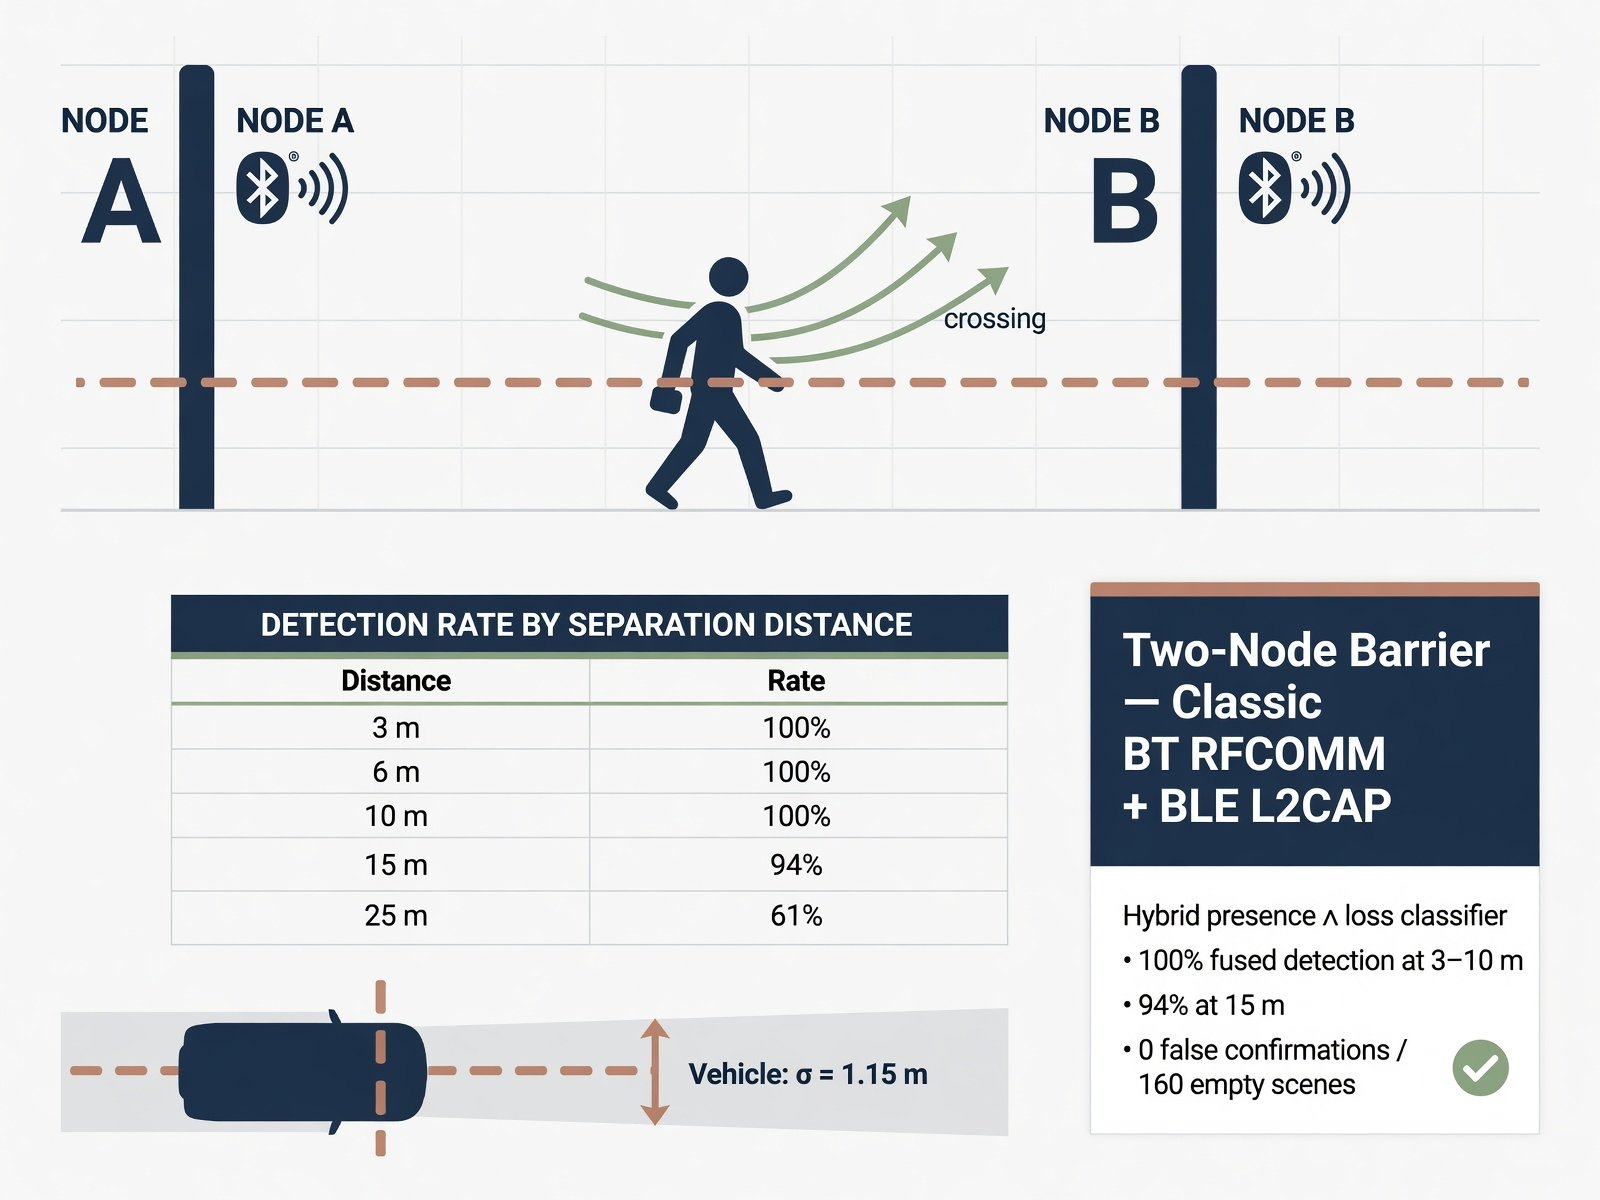
\includegraphics[width=\columnwidth]{fig_modern_06_transit.jpg}
  \caption{Two-node barrier over Classic Bluetooth RFCOMM and BLE L2CAP
  (Section~IV-F), with the vehicle lateral profile $\sigma=1.15$\,m. The rate
  panel is the app's own displayed summary: its 15\,m value is the
  BLE-channel rate and its 25\,m value the hybrid. Measured per-channel rates
  with CIs are in Section~IV-F.}
  \label{fig:transit}
\end{figure}

\subsection{Displayed versus realized accuracy}
The app displays $\hat a = 86\,\%$ for a single phone at the 10\,m preset;
the per-event confidence readout visible in Fig.~\ref{fig:sense} is the same
displayed quantity, and the envelope marked there is the live view of the
curves measured in Fig.~\ref{fig:field}(a);
realized classification on E1--E2 events within 8\,m is 79.2\,\% (38 of 48). The
Bland--Altman difference is $-6.8$\,pp (95\,\% limits of agreement
$[-18.3,\,4.7]$\,pp, mean difference $\pm1.96$\,SD of the per-session
differences; paired values accompany the release): a modest close-range overestimate, and conservative
beyond 12\,m, where the displayed value falls faster than the realized rate.
The app therefore never promises more range than the field envelope
supports.

%---------------------------------------------------------------------------
\section{Discussion}
\textbf{The role of the mesh.} A smartphone has a fixed, inherently
limited sensing range, but the mesh turns this limitation into a design
constraint that is configurable rather than an endpoint, and each node
witnesses the same crossing from a different geometry, so cross-node
agreement (within specified tolerances of $\pm5$\,s, $\pm1$ crossing, or
$\pm4$\,m) can provide independent confirmation where evidence from a link
is weakest, overlapping sensing envelopes can cover wider areas than those
accessible to one phone, and the reliability bonus favors nodes whose
observations are closest to the fused estimate; therefore, the mesh provides
three functionalities that one device cannot---confirmation, wider coverage,
and continuity---and the radius panel in Fig.~\ref{fig:mesh} displays these
functionalities as they appear in the application, while validating them
remains the goal of the upcoming multi-node campaign.

\textbf{The role of gamification.} Mesh sensing requires phones to be
deployed and participants to provide truthful measurements, so the
gamification layer is designed to encourage ongoing participation by tying
XP rewards to cross-node agreement, multi-band evidence, and proximity to
the mesh consensus, and rewards are thus based on measurement quality rather
than activity alone.

The proposed payout rules, along with participation history and badges, are
displayed in the \emph{Club} tab in Fig.~\ref{fig:club}, and the components
that were validated in this study are the single-device sensing stack and
the two-node transit counter, so the mesh and gamification layer should
therefore be seen as design contributions rather than experimentally
confirmed system capabilities; consequently, their validation will require a
distributed multi-node campaign, and the agreement-based scoring mechanism
that was proposed has not yet been protected against coordinated Sybil
attacks. Moreover, the evaluation was limited to a single handset, a single
site, dry daytime conditions, and $n=15$--20 observations per experimental
cell, which limits the extent to which the reported results can be
generalized to other devices, locations, weather conditions, and deployment
settings.

%---------------------------------------------------------------------------
\section{Conclusion}
MeshCrowd demonstrates that commodity smartphones can form a practical,
infrastructure-free sensing platform by combining BLE and dual-band Wi-Fi
measurements for passive multi-band detection, gated ranging, field-change
detection, two-node transit counting, and cooperative mesh sensing, and this
paper reports the first complete physical validation of the single-device
stack on an unmodified handset. In the field, a single phone detects
pedestrian crossings to about 16\,m (50\,\%) and sustains classification above
80\,\% inside 6\,m, detects moving vehicles to 16\,m at reduced rate, holds a
zero-BLE-false-positive budget over 30\,h of silent control, and refuses
range estimates exactly where the measured signal cannot support them. The
resulting architecture supports applications ranging from two-node pedestrian
and vehicle counting at entrances and corridors, to urban crowd and flow
monitoring, smart-mobility and roadside awareness, and emergency situational
awareness where dedicated sensing infrastructure is unavailable, with a
gamification layer linking participation and rewards to measurement
agreement.

Future evaluation will focus on the distributed multi-device campaign that
this campaign deliberately excludes: mesh confirmation and false-confirmation
rates across node densities, and gamification dynamics under sustained
participation, alongside diverse indoor and outdoor environments, device
heterogeneity, placement, multipath, interference, and battery constraints.
Mesh resilience against spoofed or adversarial reports also remains untested;
future work will address mesh integrity and incentive robustness, extending
the current agreement-based rewards toward reputation- and quality-aware
mechanisms that remain reliable under noisy, spoofed, or coordinated device
behavior.

\balance
\begin{thebibliography}{26}
\bibitem{wilson2010} J.~Wilson and N.~Patwari, ``Radio tomographic imaging with wireless networks,'' \emph{IEEE Trans.\ Mobile Comput.}, vol.~9, no.~5, pp.~621--632, May 2010.
\bibitem{januszkiewicz2018} {\L}.\,Januszkiewicz, ``Analysis of human body shadowing effect on wireless sensor networks operating in the 2.4~GHz band,'' \emph{Sensors}, vol.~18, no.~10, art.~3412, Oct.~2018, doi: 10.3390/s18103412.
\bibitem{alippi2016} C.~Alippi, M.~Bocca, G.~Boracchi, N.~Patwari, and M.~Roveri, ``RTI goes wild: Radio tomographic imaging for outdoor people detection and localization,'' \emph{IEEE Trans.\ Mobile Comput.}, vol.~15, no.~10, pp.~2585--2598, Oct.~2016.
\bibitem{li2024} Z.~Li, A.~Dubey, S.~Shen, N.~K.~Kundu, J.~Rao, and R.~Murch, ``Radio tomographic imaging with reconfigurable intelligent surfaces for integrated sensing and communication,'' \emph{IEEE Trans.\ Wireless Commun.}, vol.~23, no.~11, pp.~15784--15797, Nov.~2024.
\bibitem{wu2024} H.~Wu, C.~Cheng, C.~Peng, T.~Zhou, and T.~Chen, ``Combining transformer with a latent variable model for radio tomography based robust device-free localization,'' \emph{Comput.\ Commun.}, vol.~224, art.~108022, Oct.~2024.
\bibitem{wong2024} W.~E.~Wong, A.~H.~Wong, W.~Q.~Peh, and C.~K.~Tan, ``A high-dimensional, multi-transceiver channel state information dataset for human activity recognition,'' \emph{Data Brief}, vol.~55, art.~110673, Aug.~2024.
\bibitem{sanchez2020} D.~S\'anchez-Rodr\'iguez, M.~A.~Quintana-Su\'arez, I.~Alonso-Gonz\'alez, C.~Ley-Bosch, and J.~J.~S\'anchez-Medina, ``Fusion of channel state information and received signal strength for indoor localization using a single access point,'' \emph{Remote Sens.}, vol.~12, no.~12, art.~1995, Jun.~2020, doi: 10.3390/rs12121995.
\bibitem{ramirez2021} R.~Ramirez, C.-Y.~Huang, C.-A.~Liao, P.-T.~Lin, H.-W.~Lin, and S.-H.~Liang, ``A practice of BLE RSSI measurement for indoor positioning,'' \emph{Sensors}, vol.~21, no.~15, art.~5181, Jul.~2021, doi: 10.3390/s21155181.
\bibitem{milano2024} F.~Milano, H.~da Rocha, M.~Larocca, L.~Ferrigno, A.~Esp\'iritu Santo, J.~Salvado, and V.~Paciello, ``BLE-based indoor localization: Analysis of some solutions for performance improvement,'' \emph{Sensors}, vol.~24, no.~2, art.~376, Jan.~2024, doi: 10.3390/s24020376.
\bibitem{bai2020} L.~Bai, F.~Ciravegna, R.~Bond, and M.~Mulvenna, ``A low cost indoor positioning system based on Bluetooth Low Energy,'' \emph{IEEE Access}, vol.~8, pp.~136858--136871, 2020.
\bibitem{khan2023} D.~Khan and I.~W.-H.~Ho, ``CrossCount: Efficient device-free crowd counting by leveraging transfer learning,'' \emph{IEEE Internet Things J.}, vol.~10, no.~5, pp.~4049--4058, Mar.~2023.
\bibitem{zhou2020} R.~Zhou, Z.~Gong, X.~Lu, and Y.~Fu, ``WiFlowCount: Device-free people flow counting by exploiting Doppler effect in commodity WiFi,'' \emph{IEEE Syst.\ J.}, vol.~14, no.~4, pp.~4919--4930, Dec.~2020.
\bibitem{zhang2022} J.~Zhang, X.~Li, S.~Shi, \emph{et al.}, ``A reputation-based and privacy-preserving incentive scheme for mobile crowd sensing: A deep reinforcement learning approach,'' \emph{Wirel.\ Netw.}, 2023.
\bibitem{wang2018} J.~Wang, M.~Li, Y.~He, H.~Li, X.~Xiao, and C.~Wang, ``A blockchain based privacy-preserving incentive mechanism in crowdsensing applications,'' \emph{IEEE Access}, vol.~6, pp.~17545--17556, 2018.
\bibitem{casar2022} M.~C\"asar, T.~Pawelke, J.~Steffan, and G.~Terhorst, ``A survey on Bluetooth Low Energy security and privacy,'' \emph{Comput.\ Netw.}, vol.~202, art.~108712, Jan.~2022.
\bibitem{antonioli2020} D.~Antonioli, N.~O.~Tippenhauer, and K.~B.~Rasmussen, ``Key negotiation downgrade attacks on Bluetooth and Bluetooth Low Energy,'' \emph{ACM Trans.\ Priv.\ Secur.}, vol.~23, no.~3, art.~14, Jul.~2020.
\bibitem{cai2024} H.~Cai, ``Securing billion Bluetooth devices leveraging learning-based techniques,'' in \emph{Proc.\ AAAI Conf.\ Artif.\ Intell.\ (AAAI)}, vol.~38, no.~21, pp.~23731--23732, 2024.
\bibitem{wilson2011} J.~Wilson and N.~Patwari, ``See-through walls: Motion tracking using variance-based radio tomography networks,'' \emph{IEEE Trans. Mobile Comput.}, vol.~10, no.~5, pp.~632--643, May 2011.
\bibitem{wang2015har} W.~Wang, A.~X.~Liu, M.~Shahzad, K.~Ling, and S.~Lu, ``Understanding and modeling of WiFi signal based human activity recognition,'' in \emph{Proc. 21st Annu. Int. Conf. Mobile Comput. Netw. (MobiCom)}, 2015, pp.~65--76.
\bibitem{beresford2003} A.~R.~Beresford and F.~Stajano, ``Location privacy in pervasive computing,'' \emph{IEEE Pervasive Comput.}, vol.~2, no.~1, pp.~46--55, Jan.--Mar. 2003.
\bibitem{herrera2010} J.~C.~Herrera, D.~B.~Work, R.~Herring, X.~J.~Ban, Q.~Jacobson, and A.~M.~Bayen, ``Evaluation of traffic data obtained via GPS-enabled mobile phones: The Mobile Century field experiment,'' \emph{Transp. Res. Part C: Emerg. Technol.}, vol.~18, no.~4, pp.~568--583, Aug. 2010.
\bibitem{ma2019wifi} Y.~Ma, G.~Zhou, and S.~Wang, ``WiFi sensing with channel state information: A survey,'' \emph{ACM Comput. Surv.}, vol.~52, no.~3, art.~47, 2019, doi: 10.1145/3310194.
\bibitem{patwari2010proc} N.~Patwari and J.~Wilson, ``RF sensor networks for device-free localization: Measurements, models, and algorithms,'' \emph{Proc. IEEE}, vol.~98, no.~11, pp.~1961--1973, Nov.~2010, doi: 10.1109/JPROC.2010.2079090.
\bibitem{ryan2013woot} M.~Ryan, ``Bluetooth: With low energy comes low security,'' in \emph{Proc. 7th USENIX Workshop on Offensive Technologies (WOOT)}, 2013.
\bibitem{Brown2001Wilson} L.~D.~Brown, T.~T.~Cai, and A.~DasGupta, ``Interval estimation for a binomial proportion,'' \emph{Statist.\ Sci.}, vol.~16, no.~2, pp.~101--133, 2001.
\bibitem{Hanley1983RuleOfThree} J.~A.~Hanley and A.~Lippman-Hand, ``If nothing goes wrong, is everything all right? Interpreting zero numerators,'' \emph{JAMA}, vol.~249, no.~13, pp.~1743--1745, 1983.
\end{thebibliography}

\end{document}
